

%%%%%%%%%%%%%%%%%%%%%%%%%%%%%%%%%%%%%%%%%%%
%%%%%%  STYLE 38
%%%%%%%%%%%%%%%%%%%%%%%%%%%%%%%%%%%%%%%%%%%

\cxset{style38/.style={
 name=,
 numbering=arabic,
 number font-size=\huge,
 number font-family=\rmfamily,
 number font-weight=\normalfont,
 number before={\begin{center}},
 number position=leftname,
 chapter font-family=\sffamily,
 chapter font-weight=\normalfont,
 number after={\vspace*{6.5pt}\par},
 chapter before={},
 chapter after={},
 chapter color={black!90},
 number color=\color{black!90},
 title beforeskip={},
 title afterskip={\vspace{50pt}},
 title before=,
 title after={\par\end{center}} ,
 title font-family=\rmfamily,
 title font-color=\color{black!80},
 title font-weight=\normalfont,
 title font-size=\huge,
 chapter font-size=,
}}

\cxset{style38,
       author block=true,
       author block format=\centering}
\chapter{STAGES OF INITIATION IN THE\\ ELEUSINIAN AND\\ SAMOTHRACIAN MYSTERIES\\STYLE 38}

This style uses rules to enclose both the chapter name and number as well as the title, which necessarily needs to be rather short.
\medskip

\begin{figure}[ht]
\centering
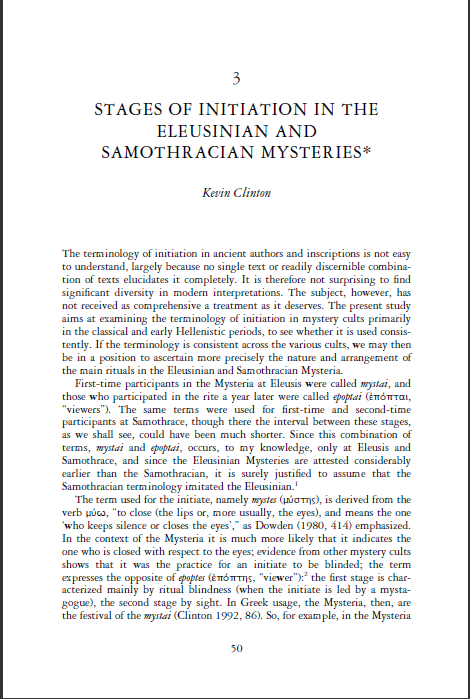
\includegraphics[width=0.6\textwidth]{./chapters/chapter38}
\end{figure}

